\documentclass[a4paper,twoside]{article}

\usepackage{xeCJK,xpinyin,graphicx}
\usepackage{geometry}%页边距
\geometry{left=2.9cm,right=2.4cm,top=2.6cm,bottom=2.6cm}
\setlength{\parindent}{3em}%缩进距离

\renewcommand{\CJKglue}{\hskip 1pt plus 0.01\baselineskip}%字间距
\linespread{1.6}%行间距
\setlength{\parskip}{1.1 \baselineskip}%段落间距

\setCJKmainfont{Adobe Song Std}

\title{般若波罗蜜多心经}
\author{}
\date{}

\begin{document}
\maketitle
\vspace{-5em}

\fontsize{14pt}{\baselineskip}\selectfont%设置字号

观自在菩萨,行深般若波罗蜜多时,照见五蕴皆空,度一切苦厄。


舍利子,色不异空,空不异色,色即是空,空即是色,受想行识,亦复如是。


舍利子,是诸法空相,不生不灭,不垢不净,不增不减。是故空中无色,无受想行识,无眼耳鼻舌身意,无色声香味触法,无眼界乃至无意识界,无无明亦无无明尽,乃至无老死,亦无老死尽,无苦集灭道,无智亦无得。


以无所得故,菩提萨埵,依般若波罗蜜多故,心无挂碍。无挂碍故,无有恐怖,远离颠倒梦想,究竟涅槃。


三世诸佛,依般若波罗蜜多故,得阿耨多罗三藐三菩提。


故知般若波罗蜜多,是大神咒,是大明咒,是无上咒,是无等等咒,能除一切苦,真实不虚。


故说般若波罗蜜多咒,即说咒曰:揭谛揭谛,波罗揭谛,波罗僧揭谛,菩提萨婆诃。
\clearpage
\vspace{5em}
\begin{pinyinscope}
观自在菩萨,行深\xpinyin{般}{bo1}\xpinyin{若}{re3}波\xpinyin{罗}{luo2}蜜多时,照见五蕴皆空,度一切苦厄。


\xpinyin{舍}{she4}利\xpinyin{子}{zi3},色不异空,空不异色,色即是空,空即是色,受想行识,亦复如是。


\xpinyin{舍}{she4}利\xpinyin{子}{zi3},是诸法空相,不生不灭,不垢不净,不增不减。是故空中无色,无受想行识,无眼耳鼻舌身意,无色声香味触法,无眼界乃至无意识界,无无明亦无无明\xpinyin{尽}{jin4},乃至无老死,亦无老死\xpinyin{尽}{jin4},无苦集灭道,无智亦无得。


以无所得故,菩提萨埵,依\xpinyin{般}{bo1}\xpinyin{若}{re3}波\xpinyin{罗}{luo2}蜜多故,心无挂碍。无挂碍故,无有恐怖,远离颠\xpinyin{倒}{dao3}梦想,究竟涅槃。


三世诸\xpinyin{佛}{fo2},依\xpinyin{般}{bo1}\xpinyin{若}{re3}波\xpinyin{罗}{luo2}蜜多故,得阿耨多\xpinyin{罗}{luo2}三藐三菩提。


故知\xpinyin{般}{bo1}\xpinyin{若}{re3}波\xpinyin{罗}{luo2}蜜多,是大神咒,是大明咒,是无上咒,是无等等咒,能除一切苦,真实不虚。


故说\xpinyin{般}{bo1}\xpinyin{若}{re3}波\xpinyin{罗}{luo2}蜜多咒,即说咒曰:揭谛揭谛,波罗揭谛,波罗僧揭谛,菩提萨婆诃。
\end{pinyinscope}

\begin{figure}[ht]
\centering
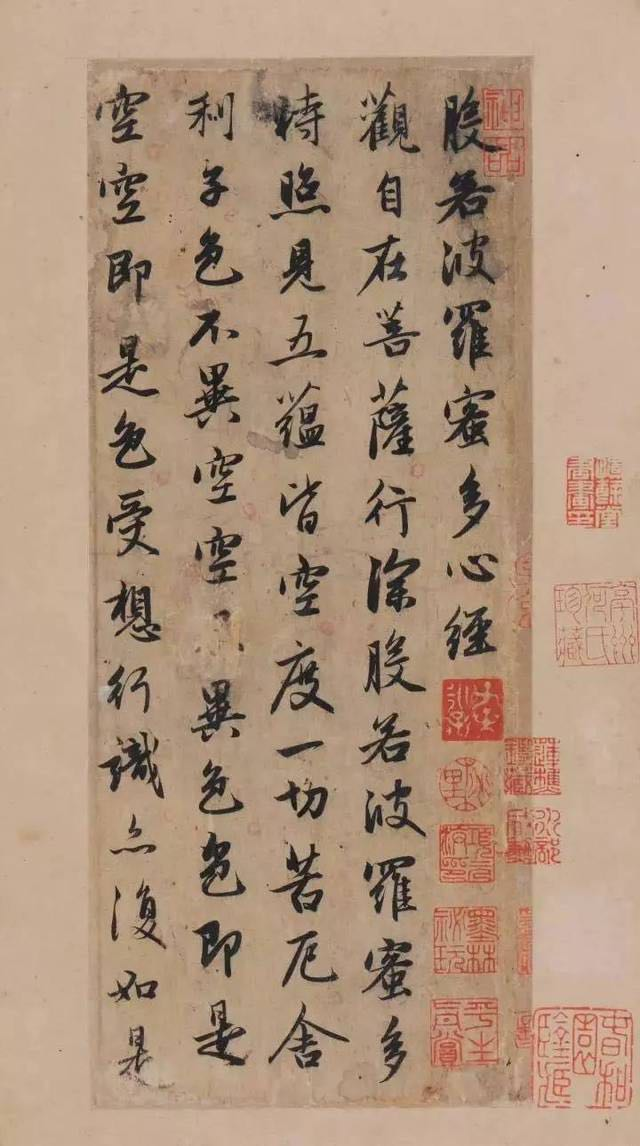
\includegraphics[width=13.2cm]{images/zhaomengfu-1}
\end{figure}
\begin{figure}[ht]
\centering
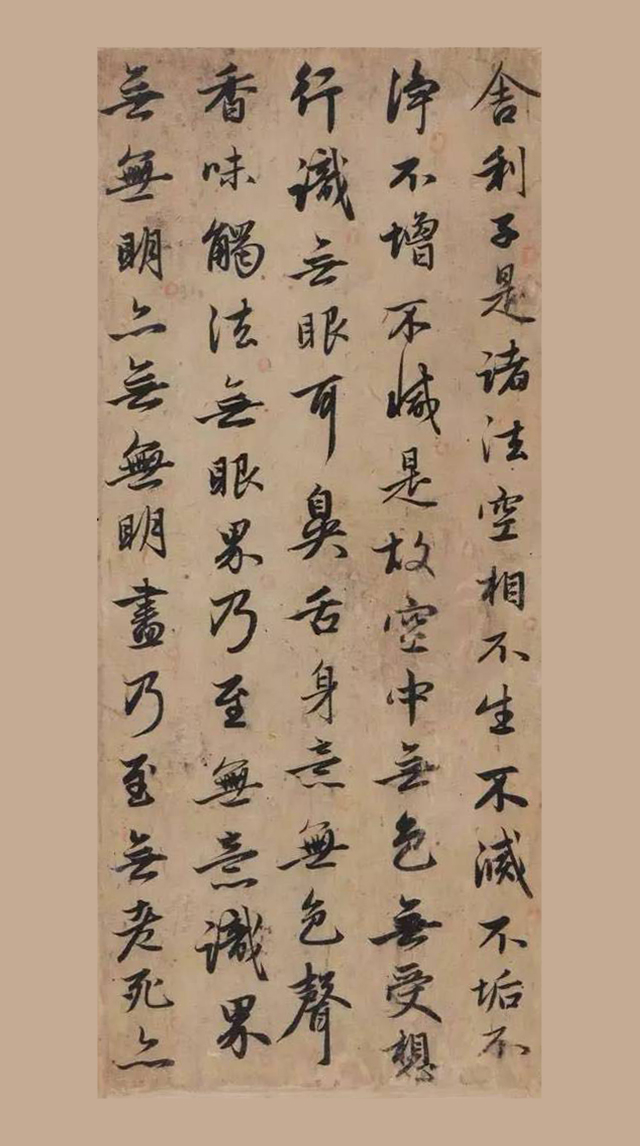
\includegraphics[width=13.2cm]{images/zhaomengfu-2}
\end{figure}
\begin{figure}[ht]
\centering
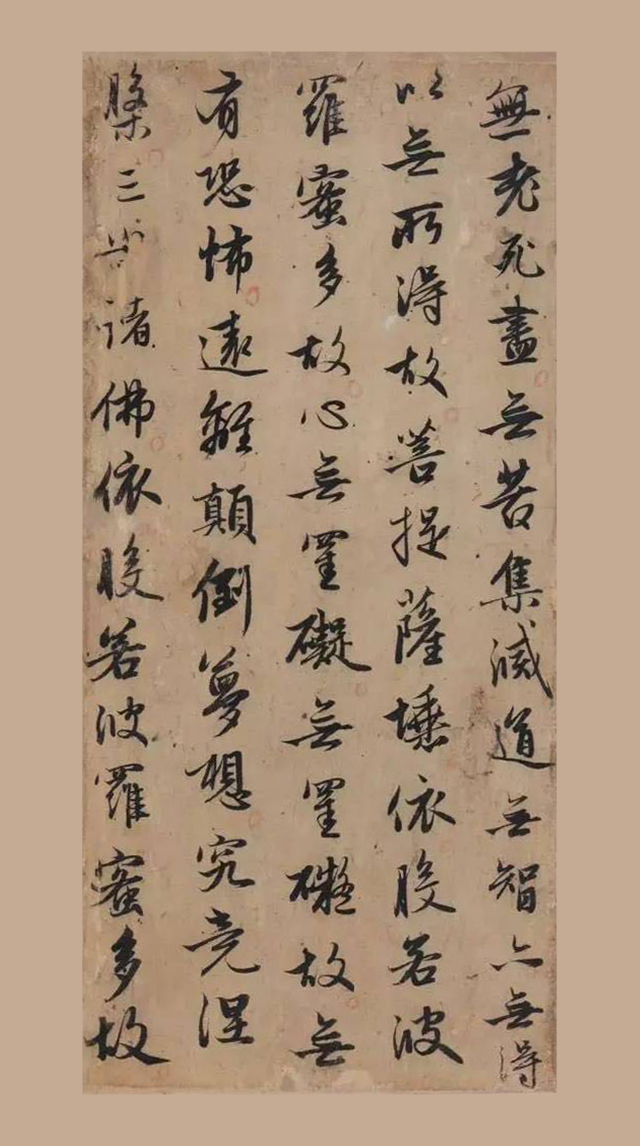
\includegraphics[width=13.2cm]{images/zhaomengfu-3}
\end{figure}
\begin{figure}[ht]
\centering
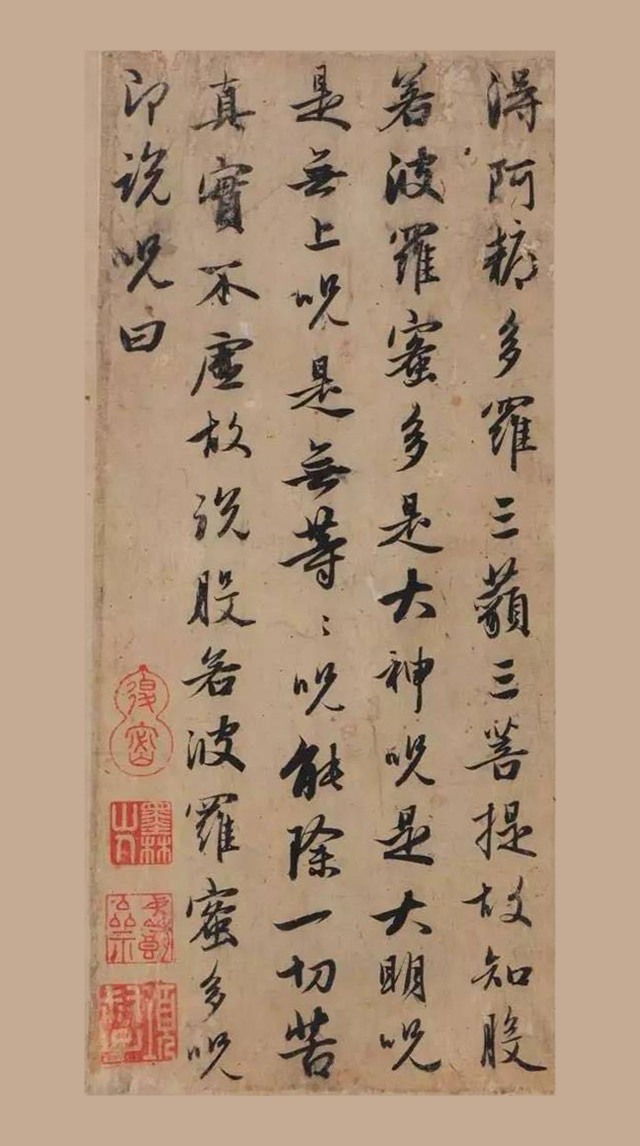
\includegraphics[width=13.2cm]{images/zhaomengfu-4}
\end{figure}
\begin{figure}[ht]
\centering
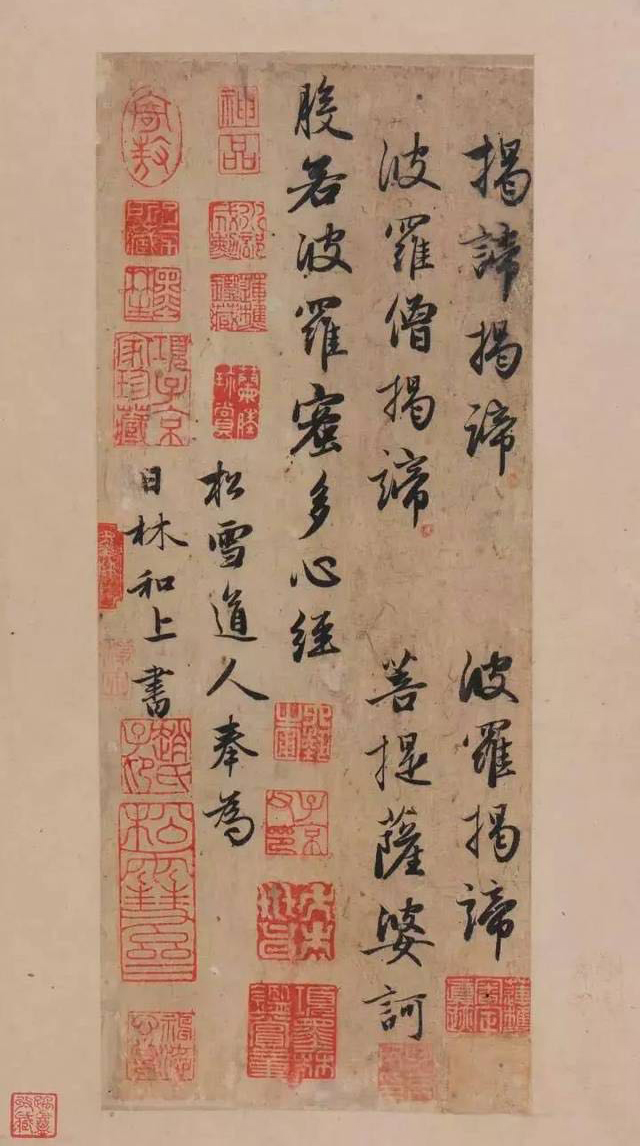
\includegraphics[width=13.2cm]{images/zhaomengfu-5}
\end{figure}
\cleardoublepage

\begin{figure}[ht]
\centering
\includegraphics[width=11.6cm]{images/ouyangxun-1}
\end{figure}
\begin{figure}[ht]
\centering
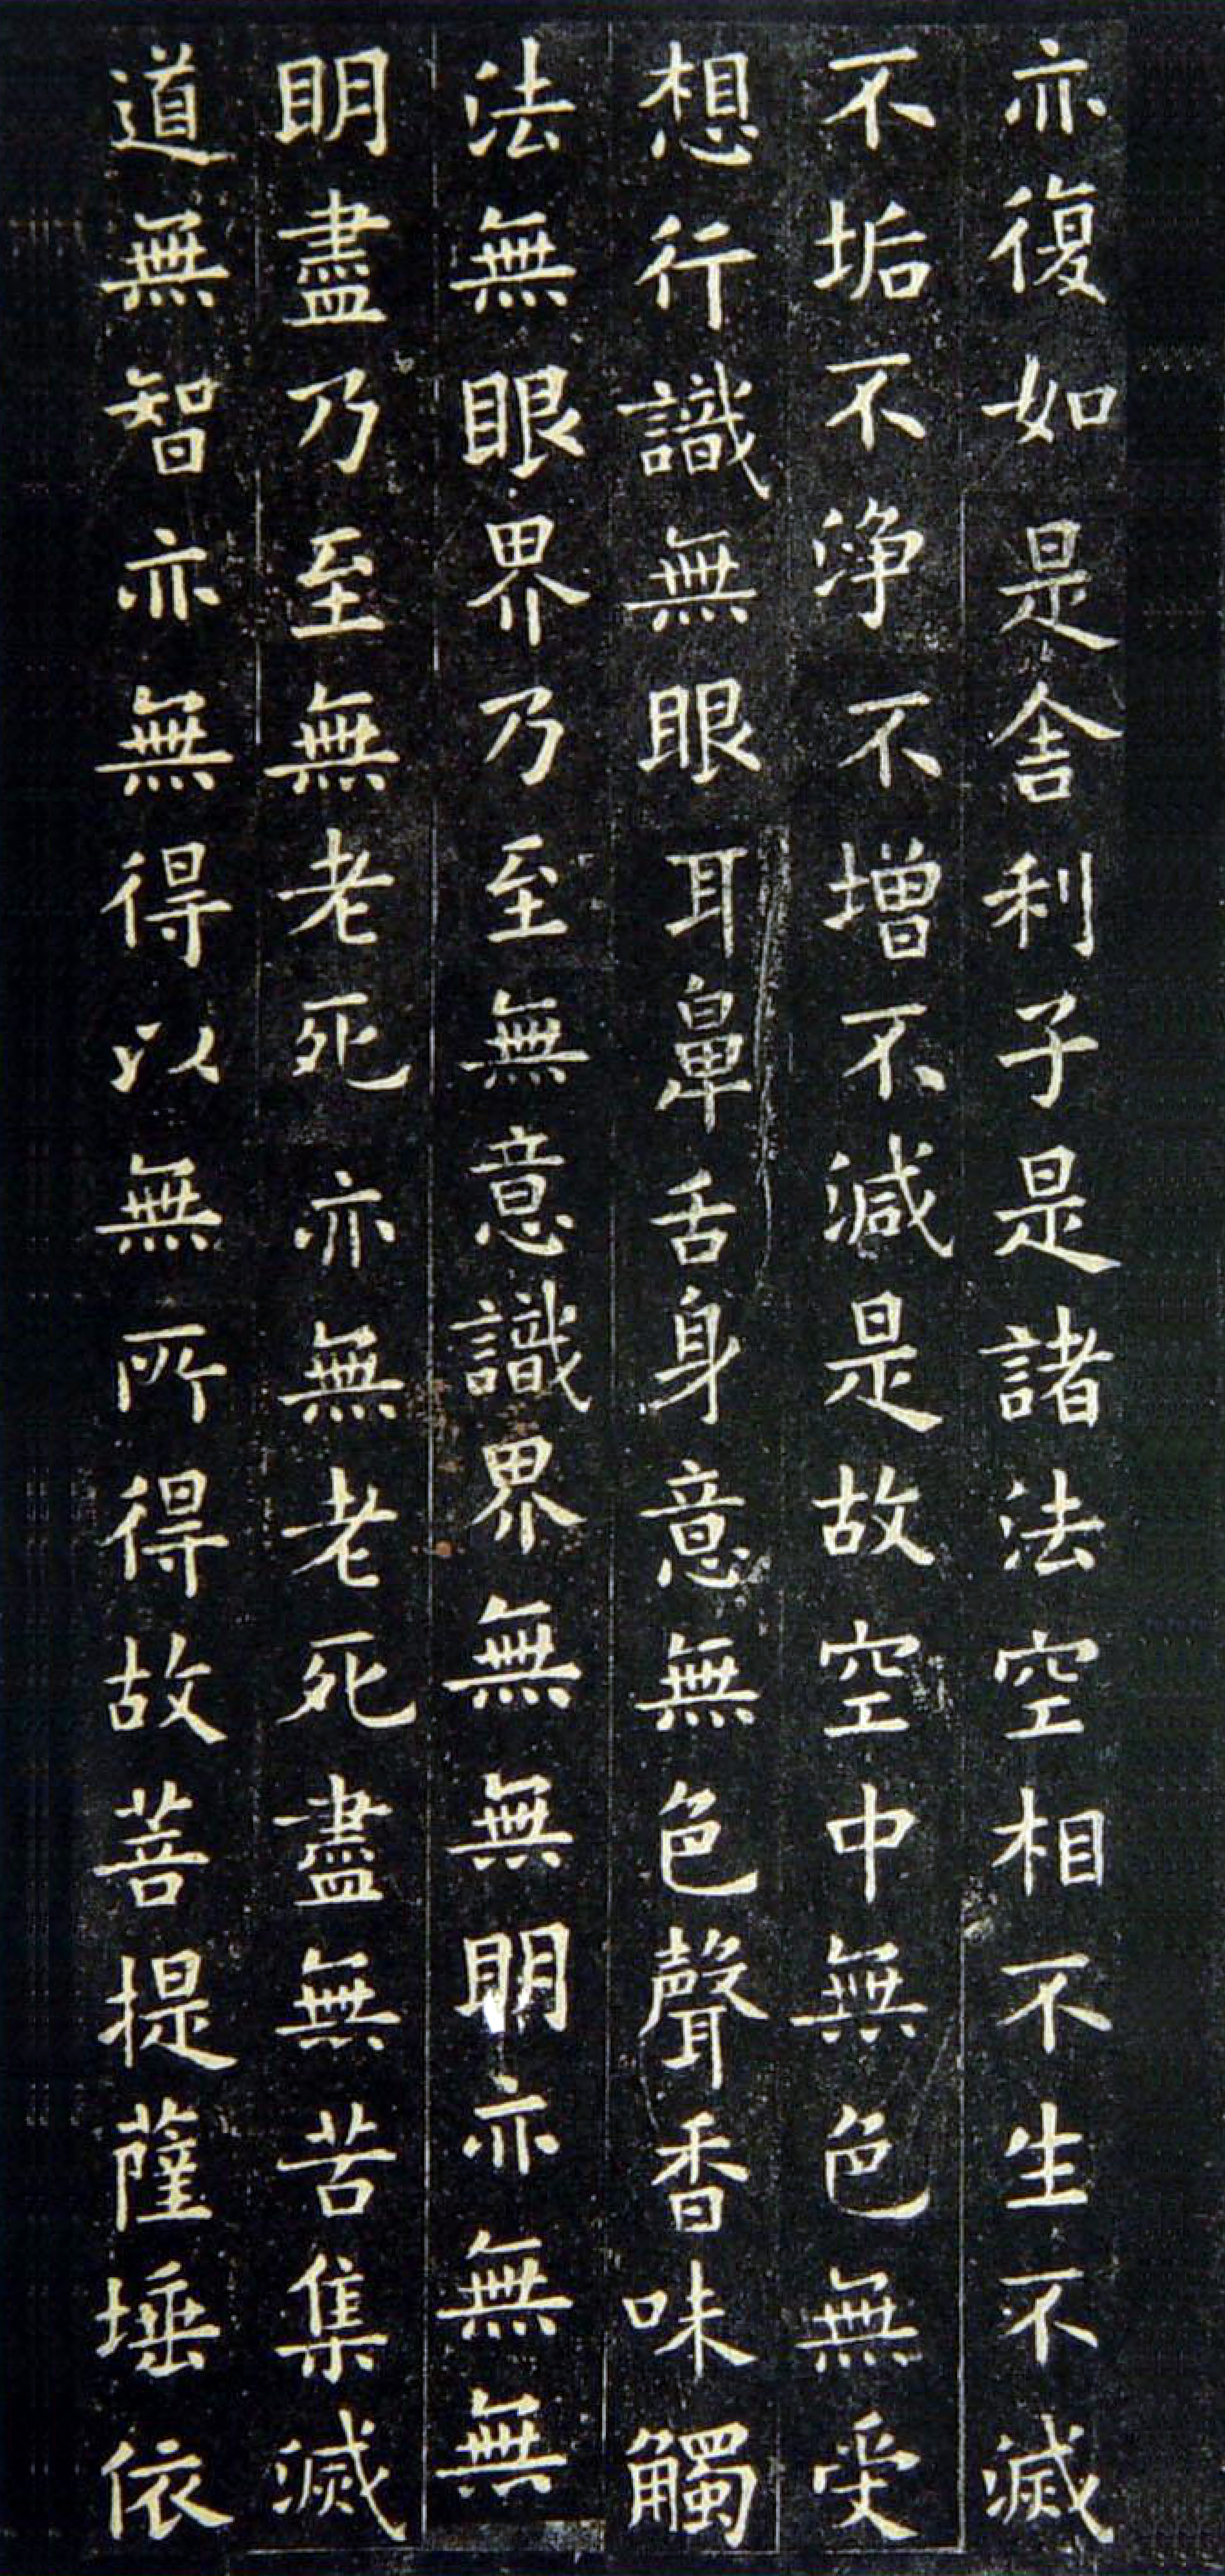
\includegraphics[width=11.6cm]{images/ouyangxun-2}
\end{figure}
\begin{figure}[ht]
\centering
\includegraphics[width=11.6cm]{images/ouyangxun-3}
\end{figure}
\begin{figure}[ht]
\centering
\includegraphics[width=11.6cm]{images/ouyangxun-4}
\end{figure}
\cleardoublepage

\begin{figure}[ht]
\centering
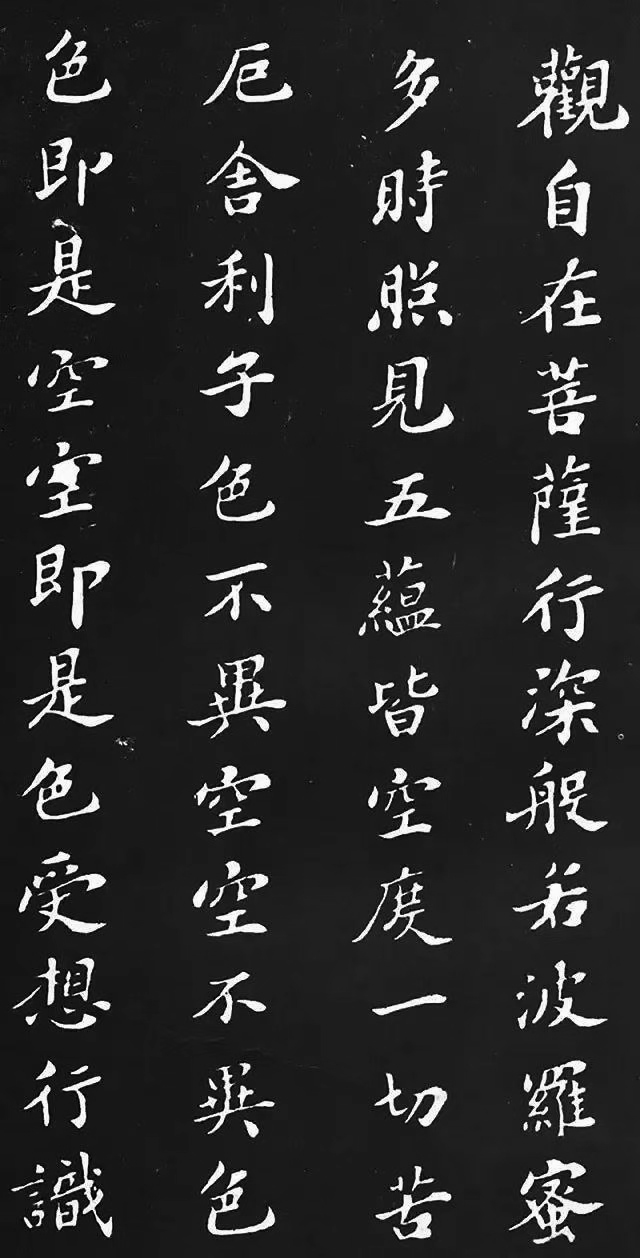
\includegraphics[width=12.2cm]{images/sushi-1}
\end{figure}
\begin{figure}[ht]
\centering
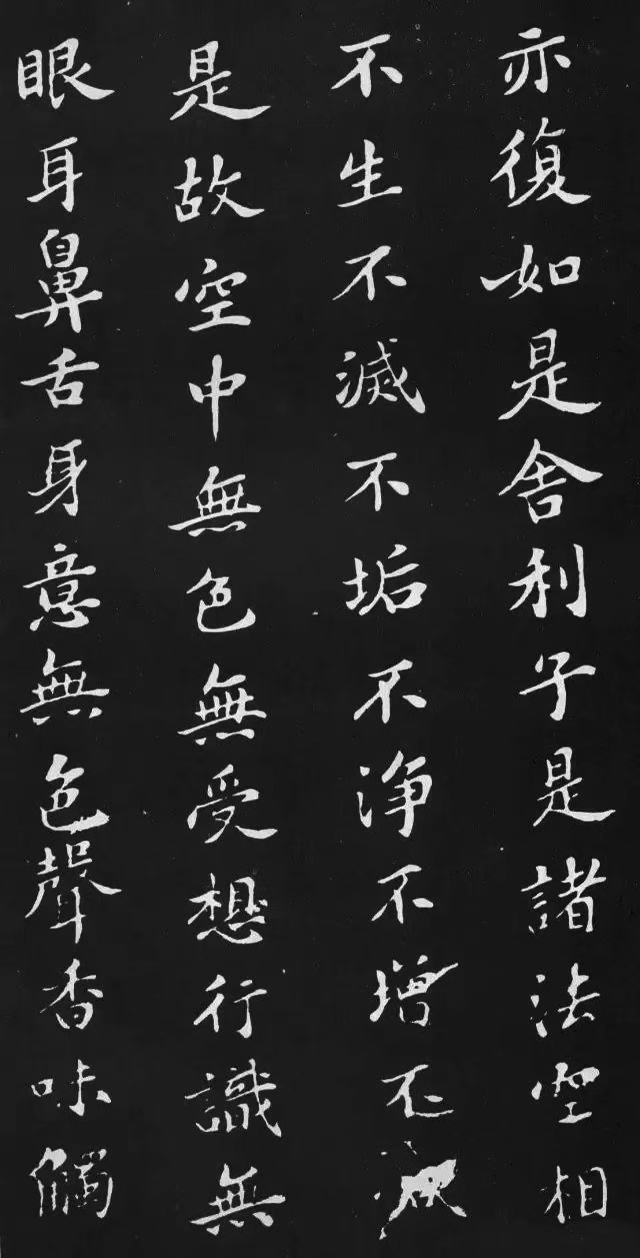
\includegraphics[width=12.2cm]{images/sushi-2}
\end{figure}
\begin{figure}[ht]
\centering
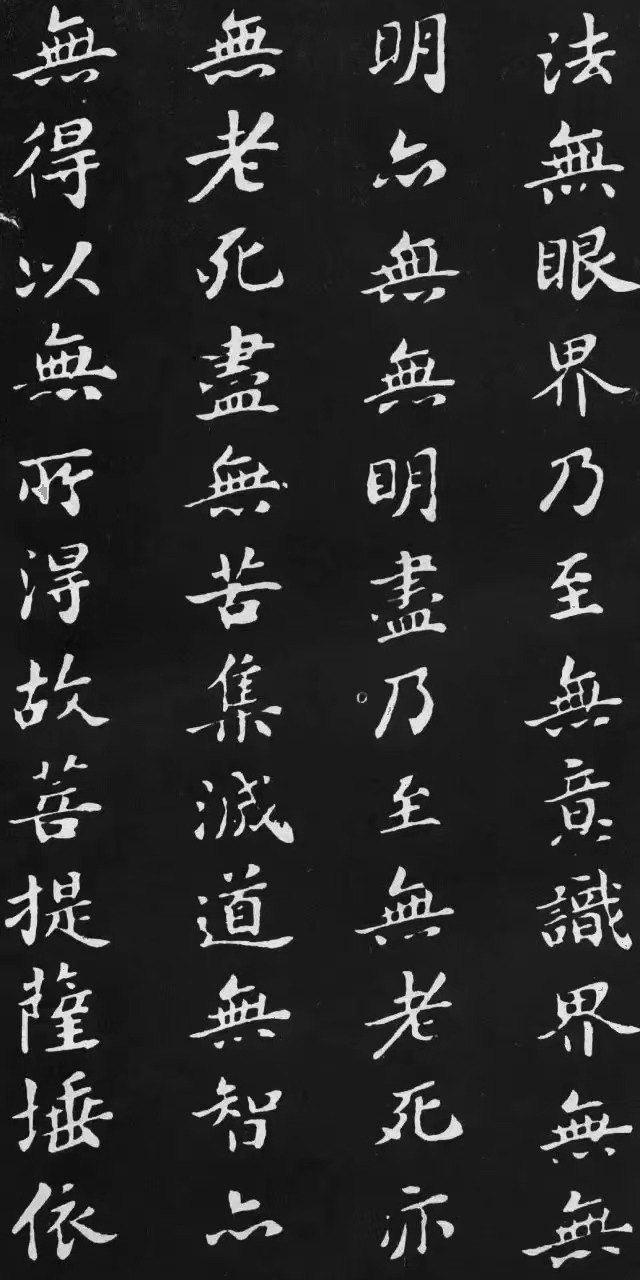
\includegraphics[width=12.2cm]{images/sushi-3}
\end{figure}
\begin{figure}[ht]
\centering
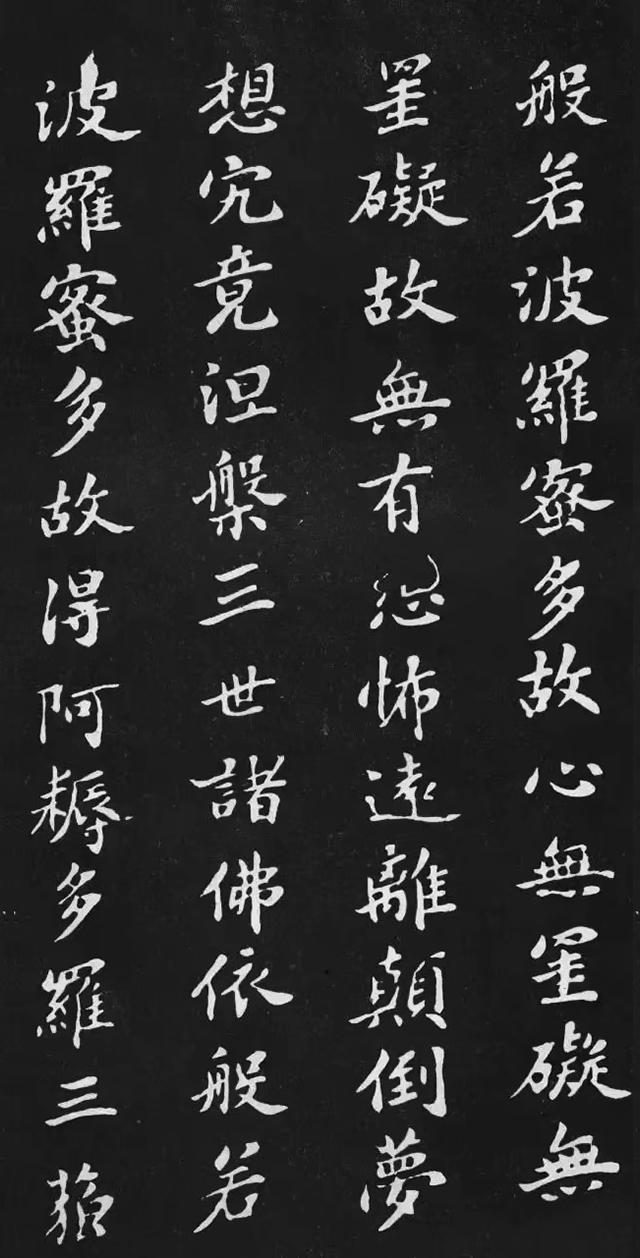
\includegraphics[width=12.2cm]{images/sushi-4}
\end{figure}
\begin{figure}[ht]
\centering
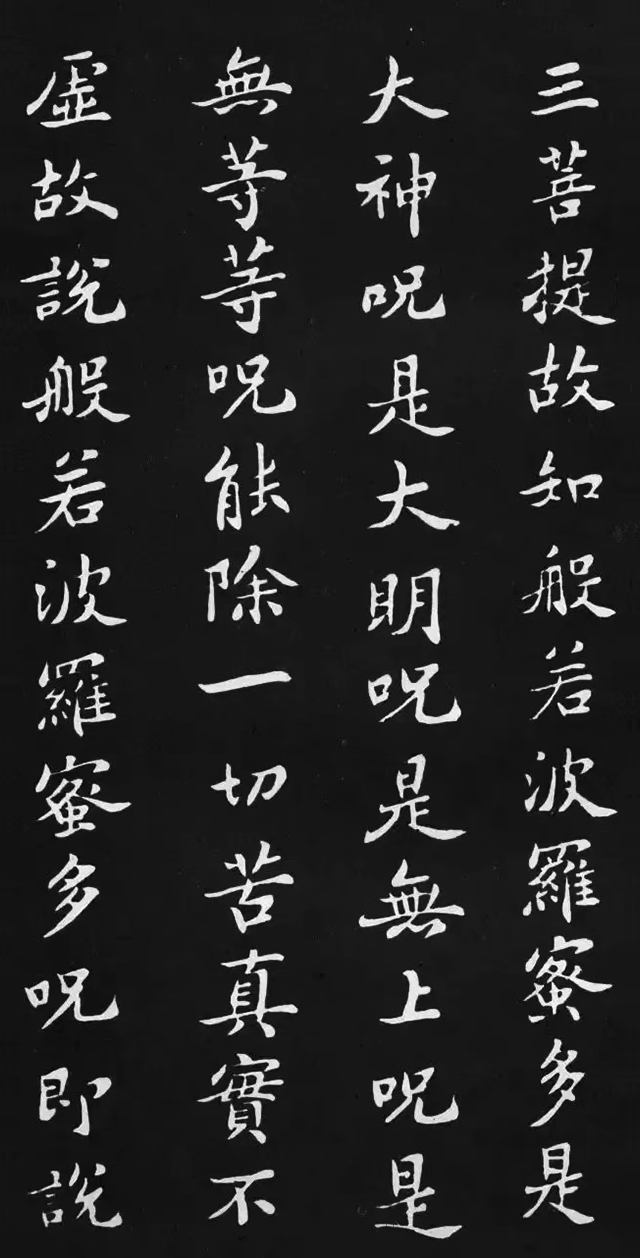
\includegraphics[width=12.2cm]{images/sushi-5}
\end{figure}
\begin{figure}[ht]
\centering
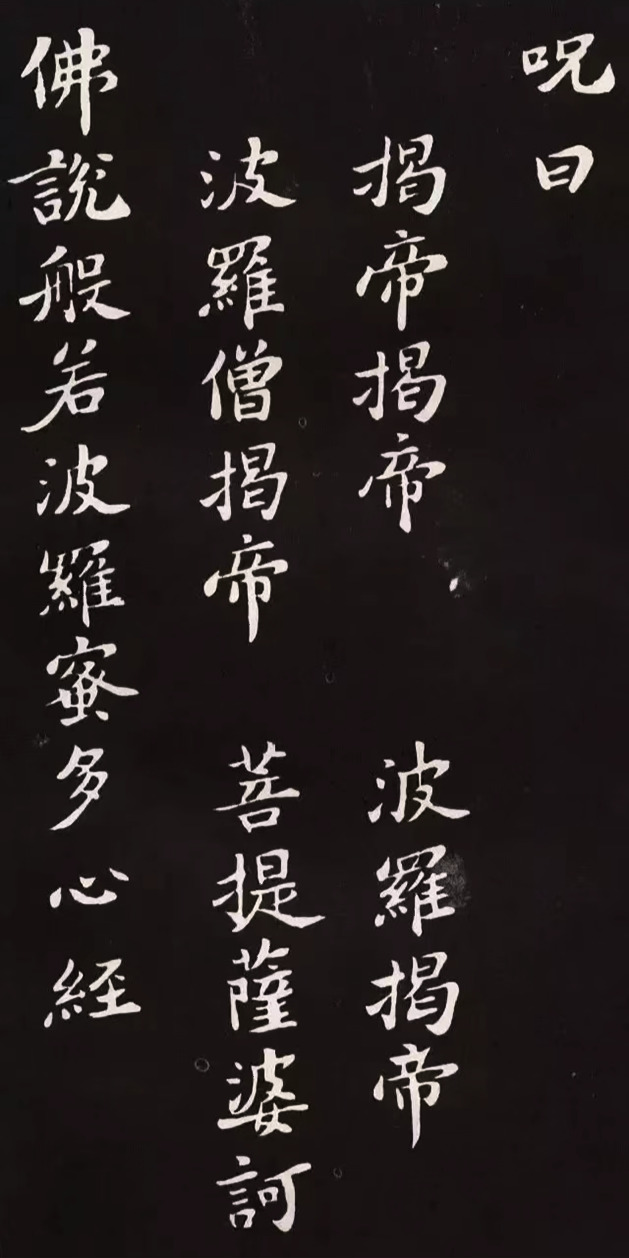
\includegraphics[width=12.2cm]{images/sushi-6}
\end{figure}
\begin{figure}[ht]
\centering
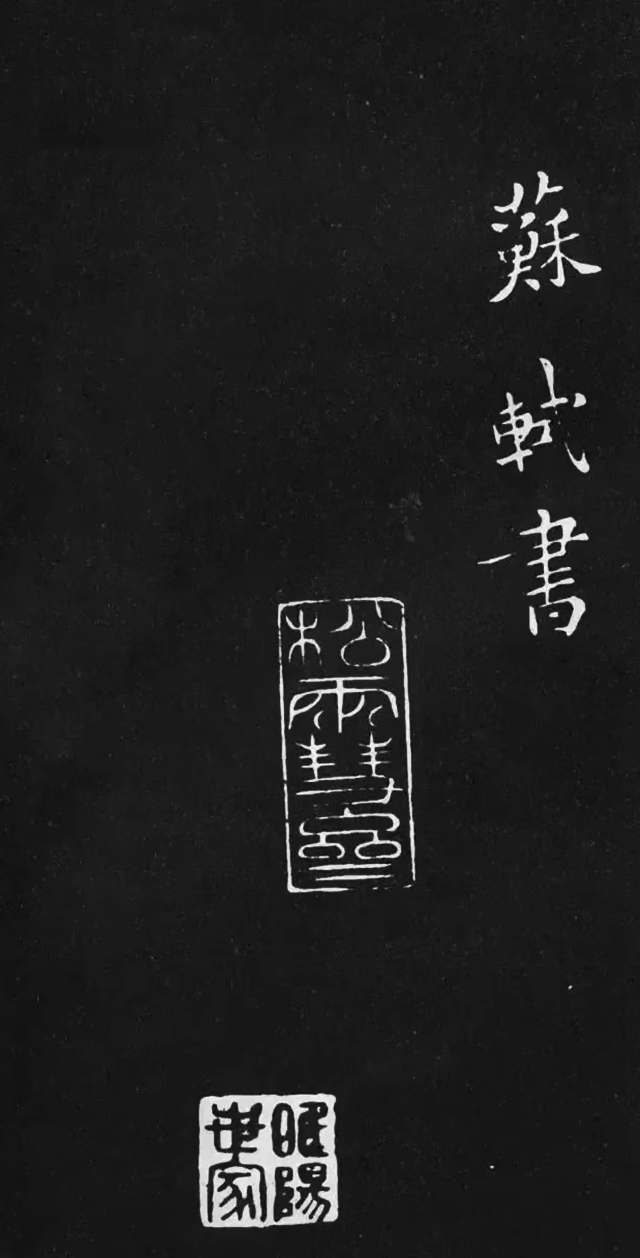
\includegraphics[width=12.2cm]{images/sushi-7}
\end{figure}
\cleardoublepage

\begin{figure}[ht]
\centering
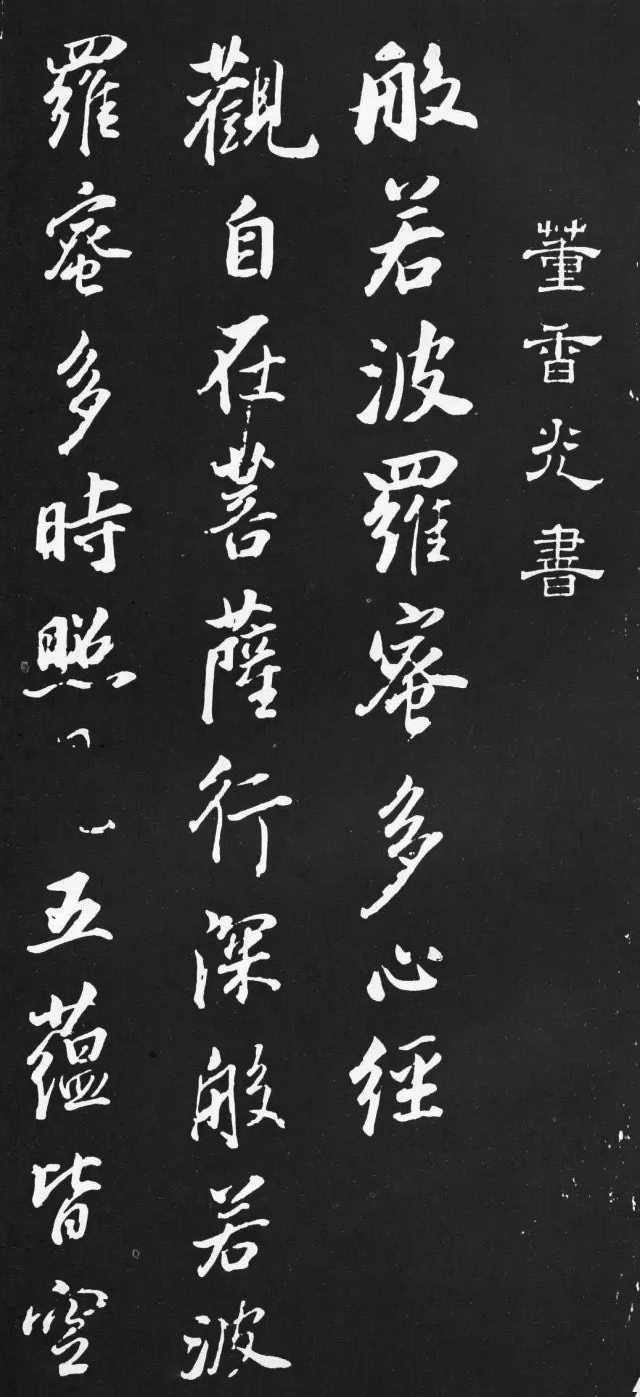
\includegraphics[width=11.2cm]{images/dongqichang-1}
\end{figure}
\begin{figure}[ht]
\centering
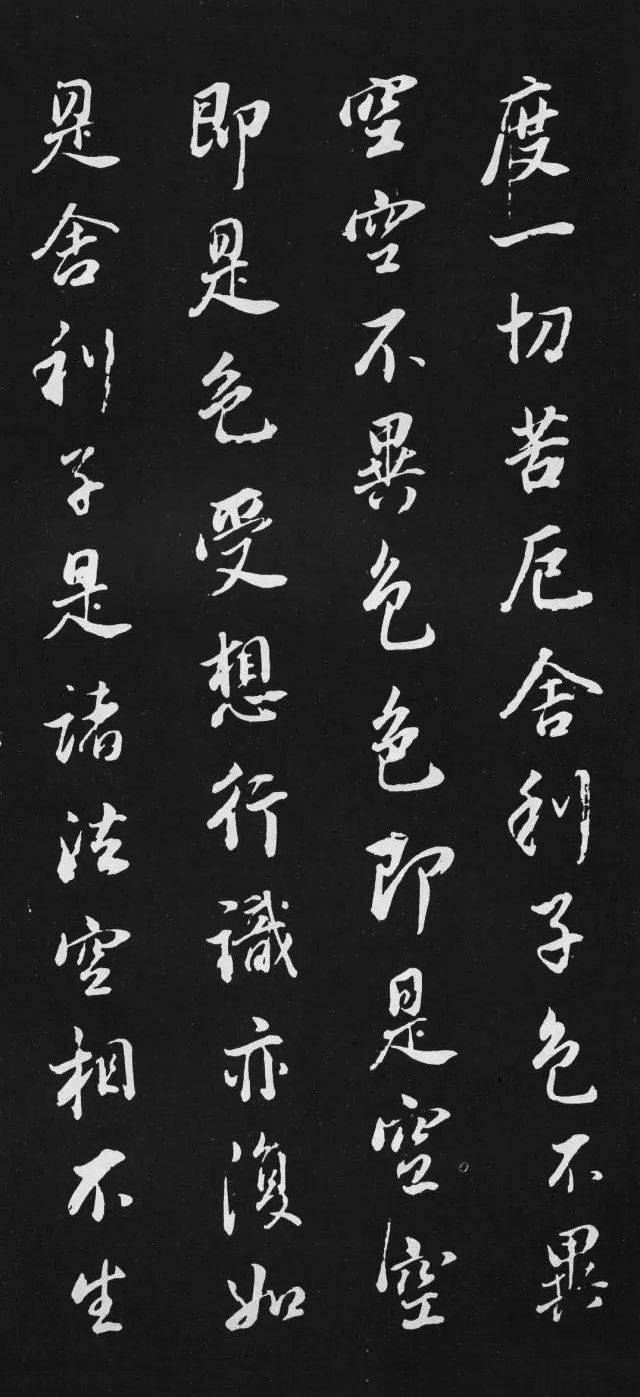
\includegraphics[width=11.2cm]{images/dongqichang-2}
\end{figure}
\begin{figure}[ht]
\centering
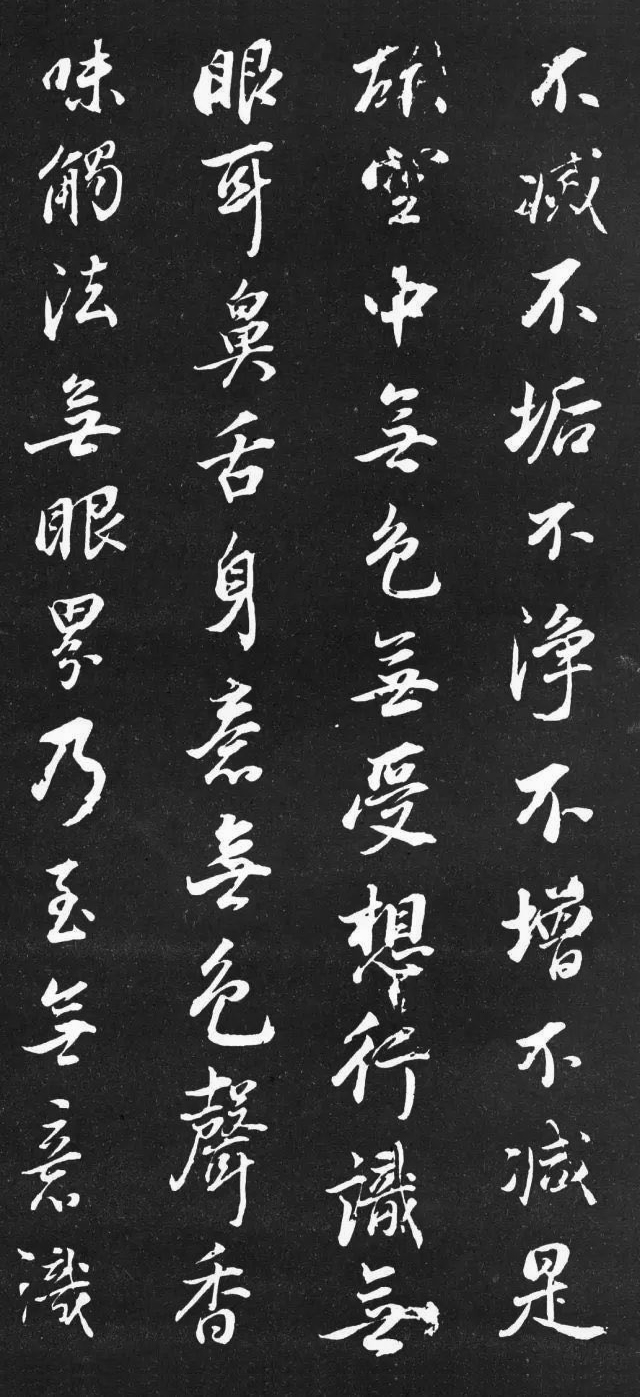
\includegraphics[width=11.2cm]{images/dongqichang-3}
\end{figure}
\begin{figure}[ht]
\centering
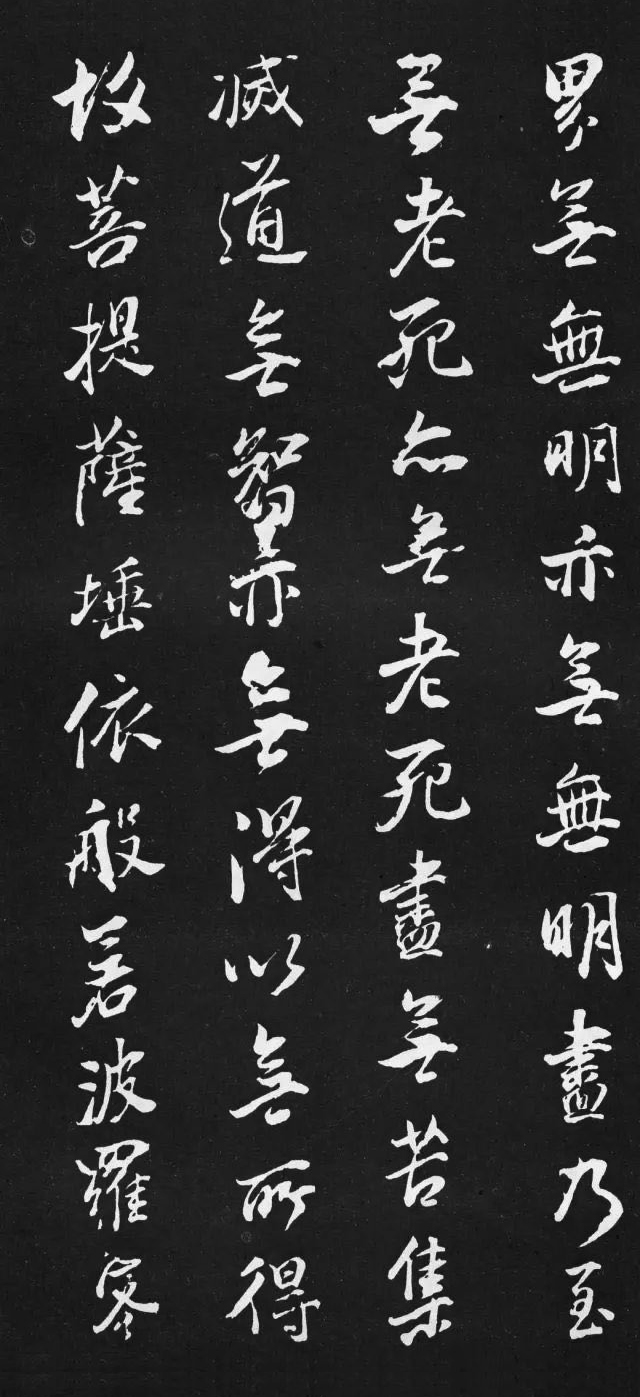
\includegraphics[width=11.2cm]{images/dongqichang-4}
\end{figure}
\begin{figure}[ht]
\centering
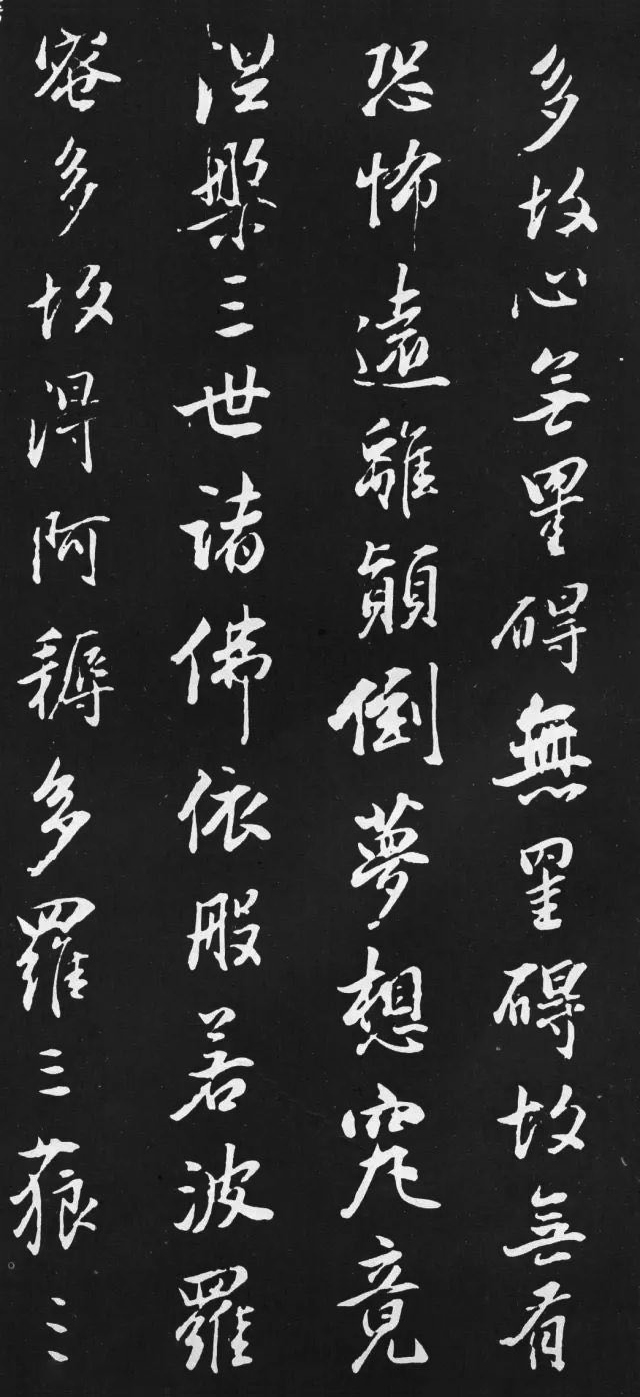
\includegraphics[width=11.2cm]{images/dongqichang-5}
\end{figure}
\begin{figure}[ht]
\centering
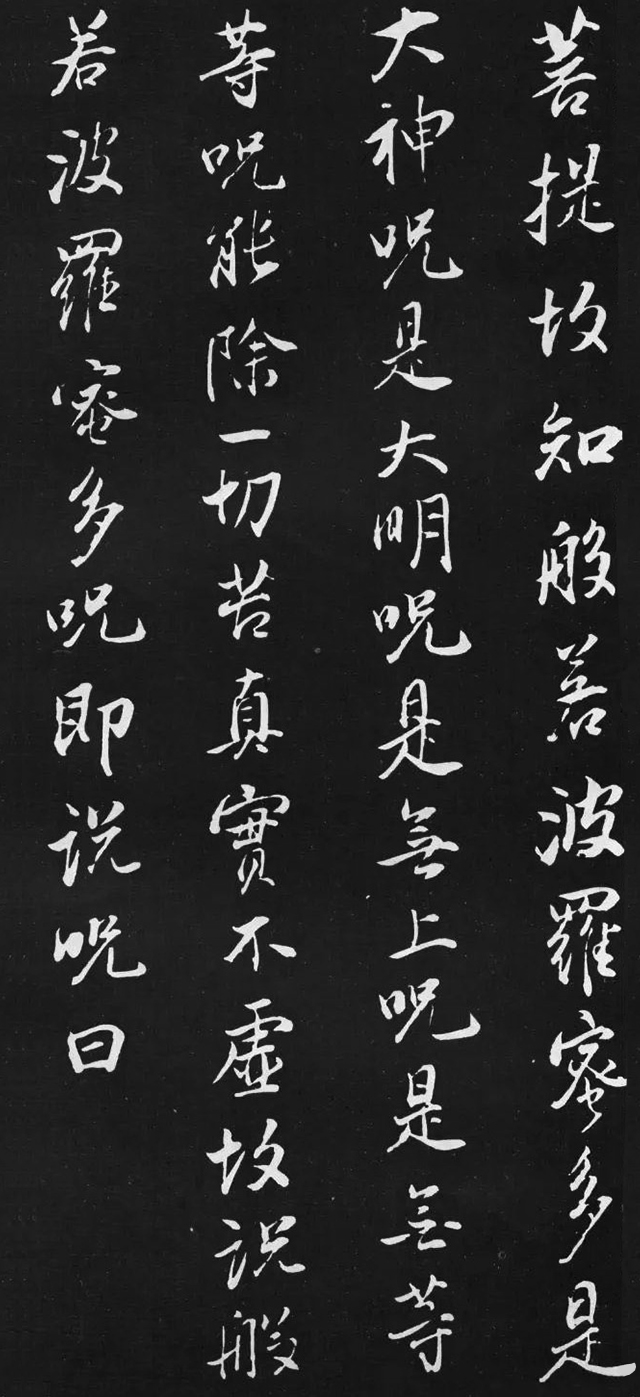
\includegraphics[width=11.2cm]{images/dongqichang-6}
\end{figure}
\begin{figure}[ht]
\centering
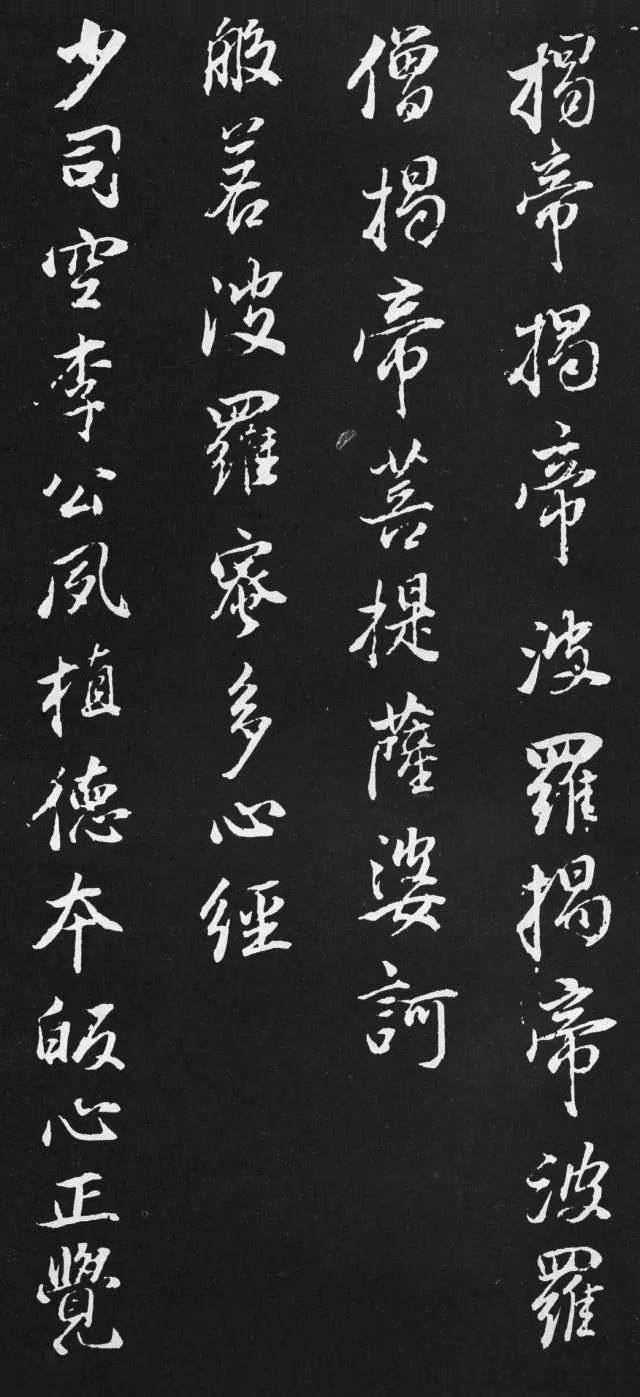
\includegraphics[width=11.2cm]{images/dongqichang-7}
\end{figure}
\begin{figure}[ht]
\centering
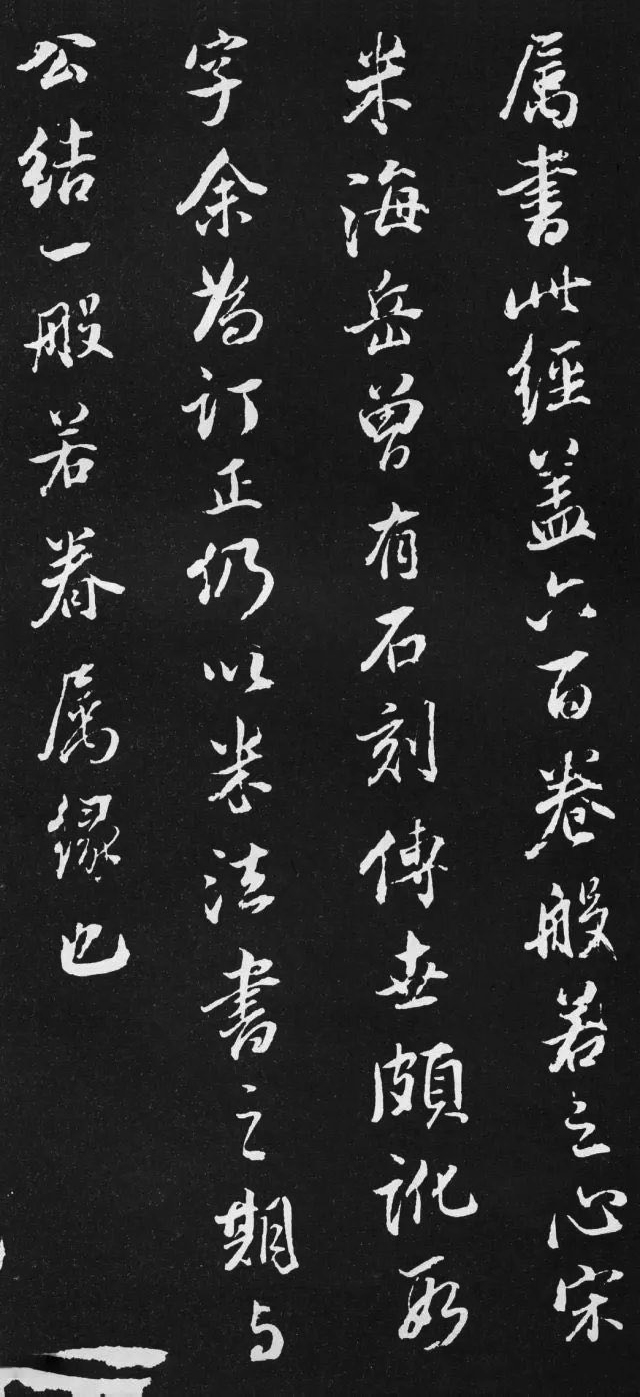
\includegraphics[width=11.2cm]{images/dongqichang-8}
\end{figure}
\begin{figure}[ht]
\centering
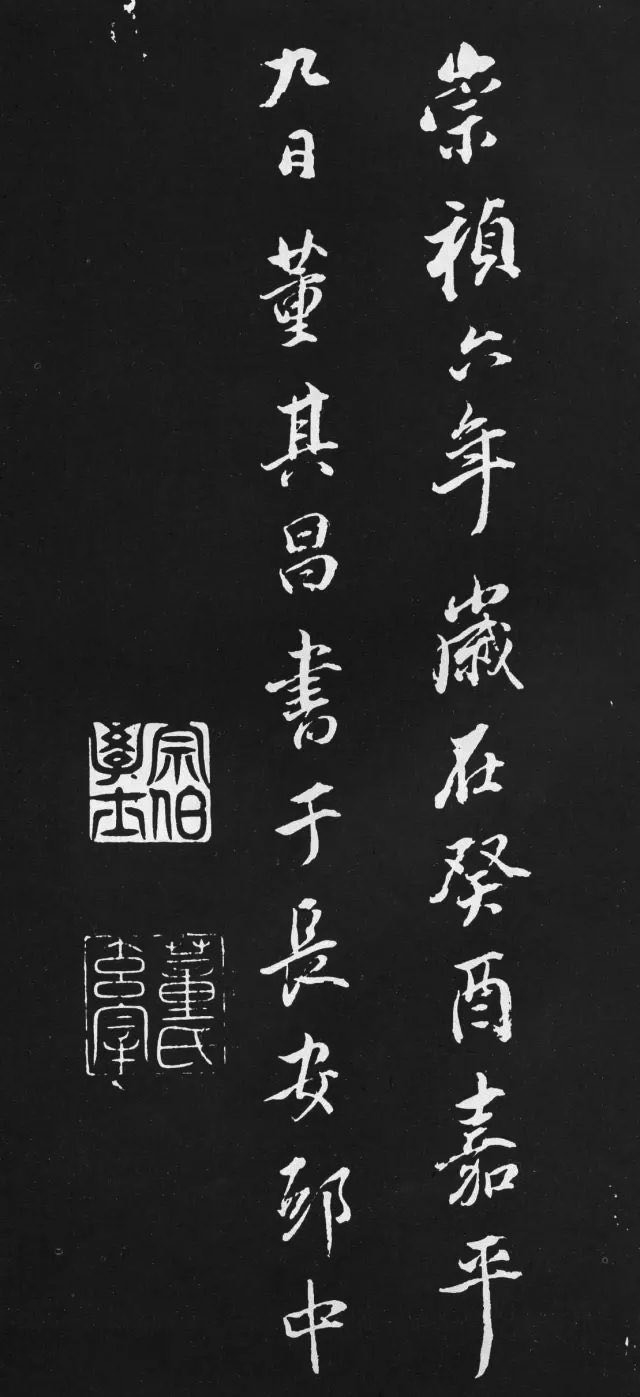
\includegraphics[width=11.2cm]{images/dongqichang-9}
\end{figure}
\cleardoublepage

\begin{figure}[ht]
\centering
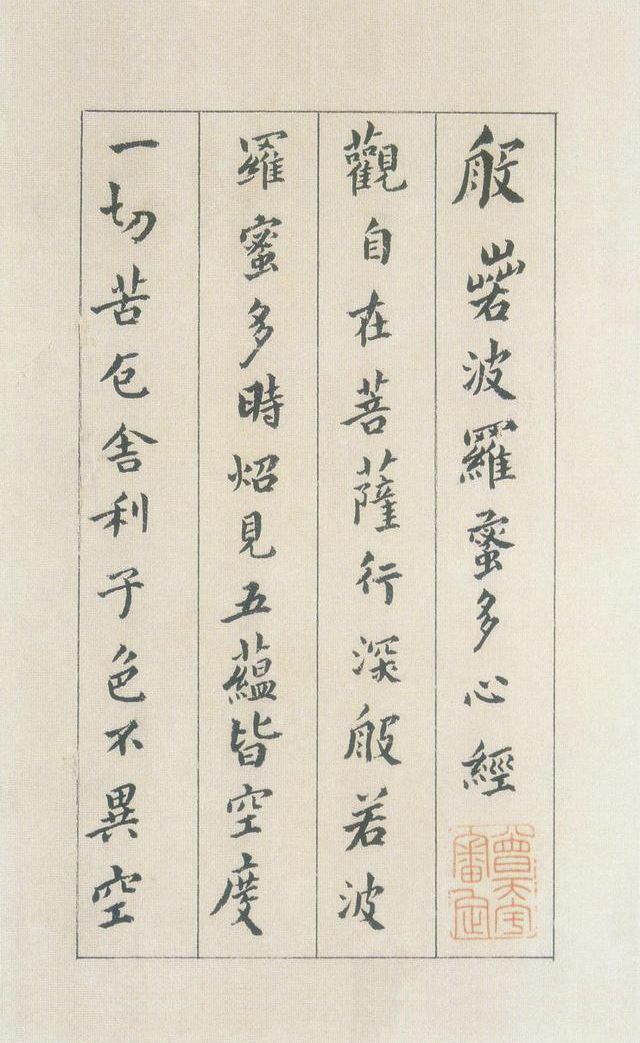
\includegraphics[width=13.8cm]{images/fushan-1}
\end{figure}
\begin{figure}[ht]
\centering
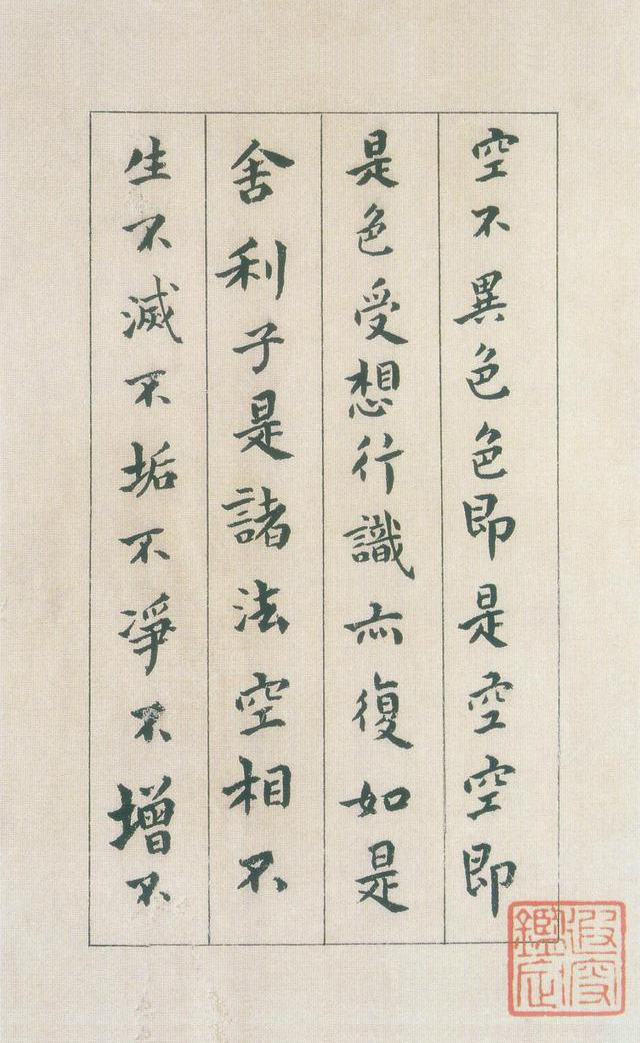
\includegraphics[width=13.8cm]{images/fushan-2}
\end{figure}
\begin{figure}[ht]
\centering
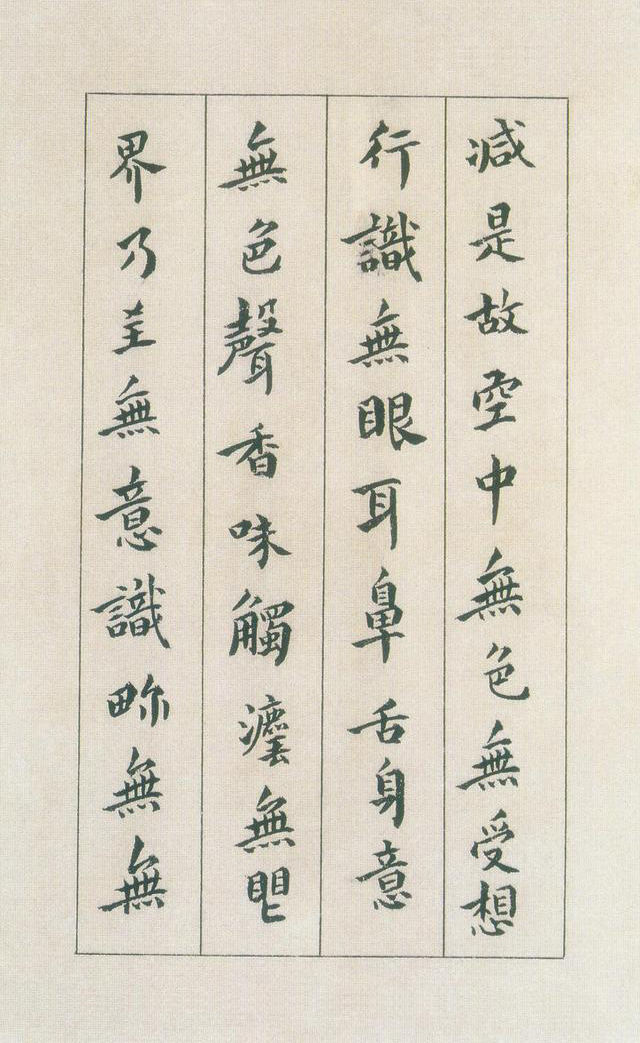
\includegraphics[width=13.8cm]{images/fushan-3}
\end{figure}
\begin{figure}[ht]
\centering
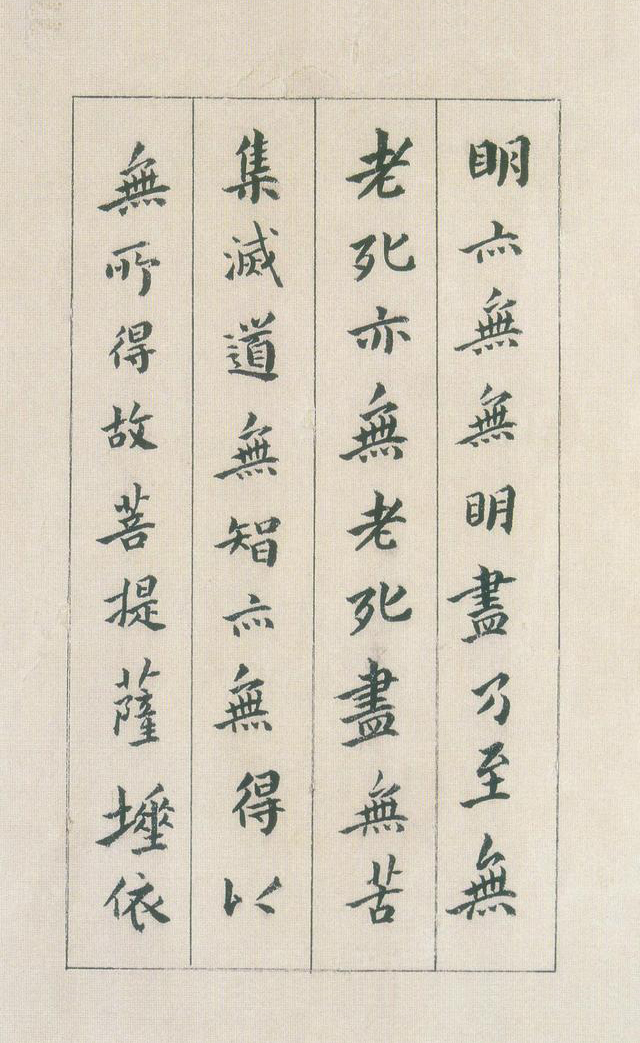
\includegraphics[width=13.8cm]{images/fushan-4}
\end{figure}
\begin{figure}[ht]
\centering
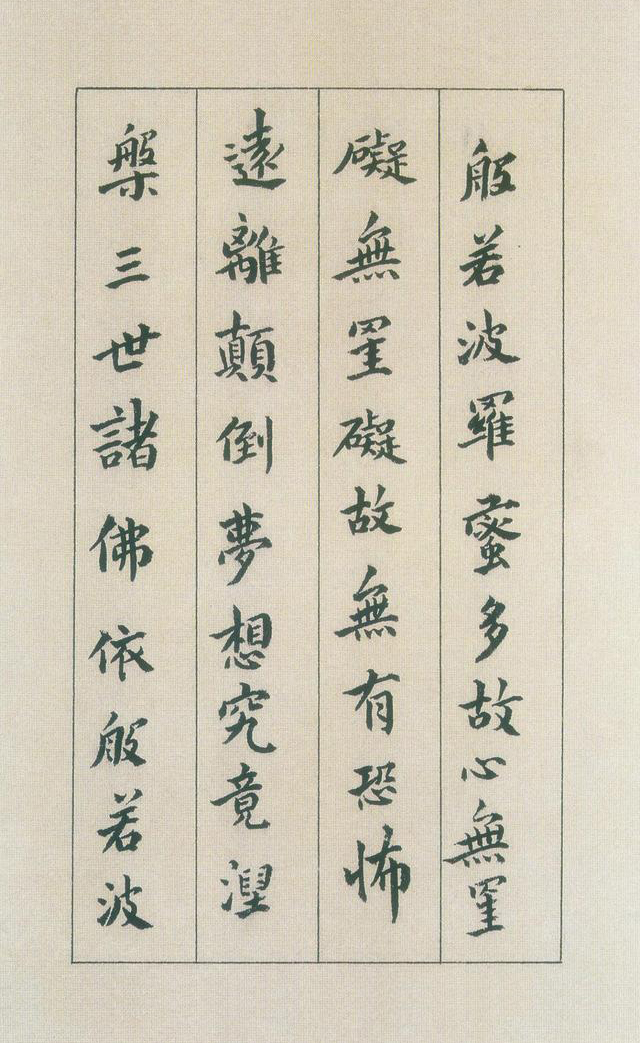
\includegraphics[width=13.8cm]{images/fushan-5}
\end{figure}
\begin{figure}[ht]
\centering
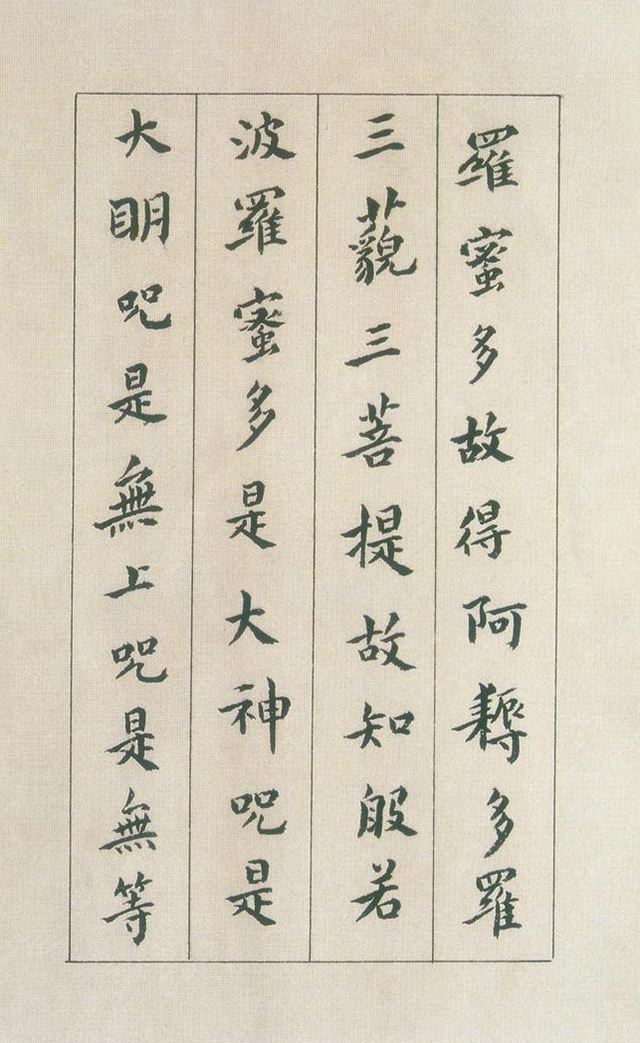
\includegraphics[width=13.8cm]{images/fushan-6}
\end{figure}
\begin{figure}[ht]
\centering
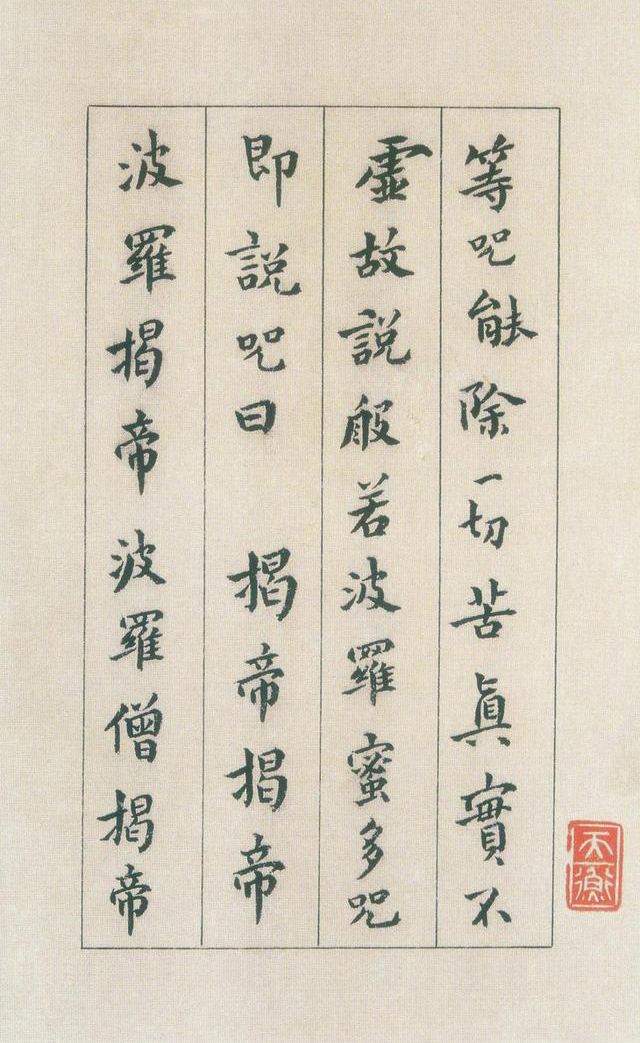
\includegraphics[width=13.8cm]{images/fushan-7}
\end{figure}
\begin{figure}[ht]
\centering
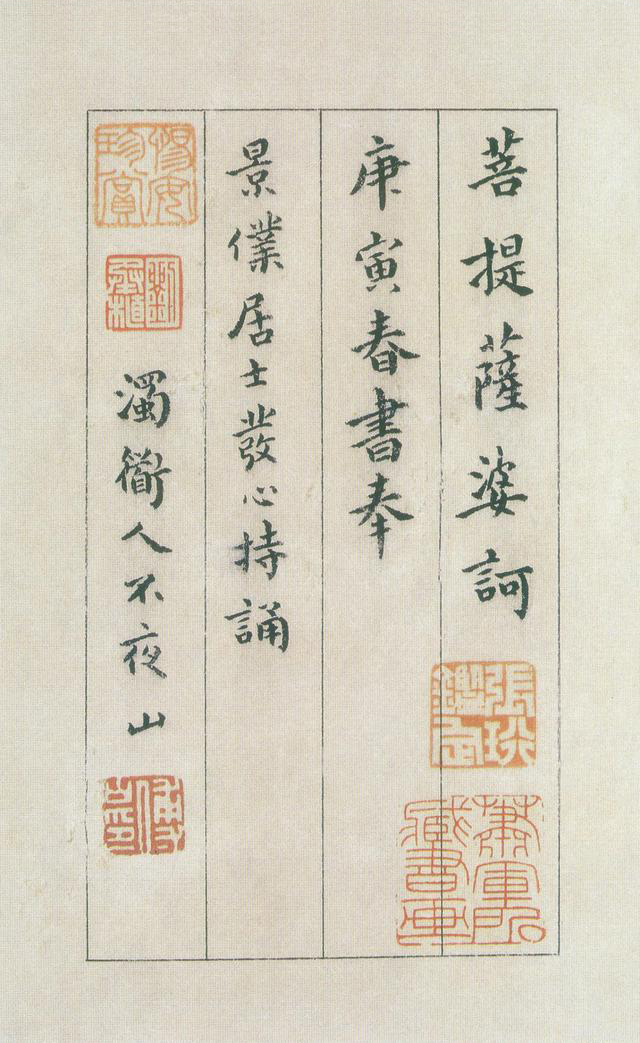
\includegraphics[width=13.8cm]{images/fushan-8}
\end{figure}
\end{document}
